\chapter{Correlations between random variables}\label{Section_3.4}

\section{General description}\label{Section_3.4.2.1}
In \Aref{Section_3.3} the procedure for applying statistical distribution functions of random variables was explained. In the explanation, the $X$-variables were assumed to be mutually independent for the sake of simplicity. In many cases, however, random variables of hydraulic load models are not mutually independent. For instance, wind speed and sea water level are correlated and the same generally can be stated for river discharges of adjacent rivers (such as the Rhine and Meuse in the Netherlands). Correlation between two random variables $X_1$ and $X_2$ needs to be taken into account in probabilistic analysis because they influence the probability of failure of the component or system under consideration.

The general approach for modeling correlation between two random variables $X_1$ and $X_2$ is to first generate correlated samples $u_{1,cor}$ and $u_{2,cor}$ from standard normally distributed variables $U_{1,cor}$ and $U_{2,cor}$.\footnote{ Note that $u_1$ and $u_2$ are strictly speaking only ''realizations'' if a Monte Carlo procedure is applied, see \Aref{Section_2.3}. For methods like FORM and numerical integration, $u_1$ and $u_2$ are strategically selected values, not samples from a simulation of a distribution function. However, this fundamental difference in interpretation of $u_1$ and $u_2$ has no influence on the applied methods as described in the current section.} The correlated samples, or realizations, are subsequently translated into realizations $x_1$ and $x_2$ of ''real world'' variables $X_1$ and $X_2$ through application of the procedure of \Aref{Section_3.3} (i.e. through application of the inverse CDF's of variables $X_1$ and $X_2$). The procedure is depicted in the figure below. The horizontal part of this figure is the exact same procedure as depicted in \Fref{fig:Figure_3.3} and explained in \Aref{Section_3.3}. The correlation model can therefore be considered as a pre-processing of the procedure in which the distribution functions are applied.

\begin{figure}[H]\centering
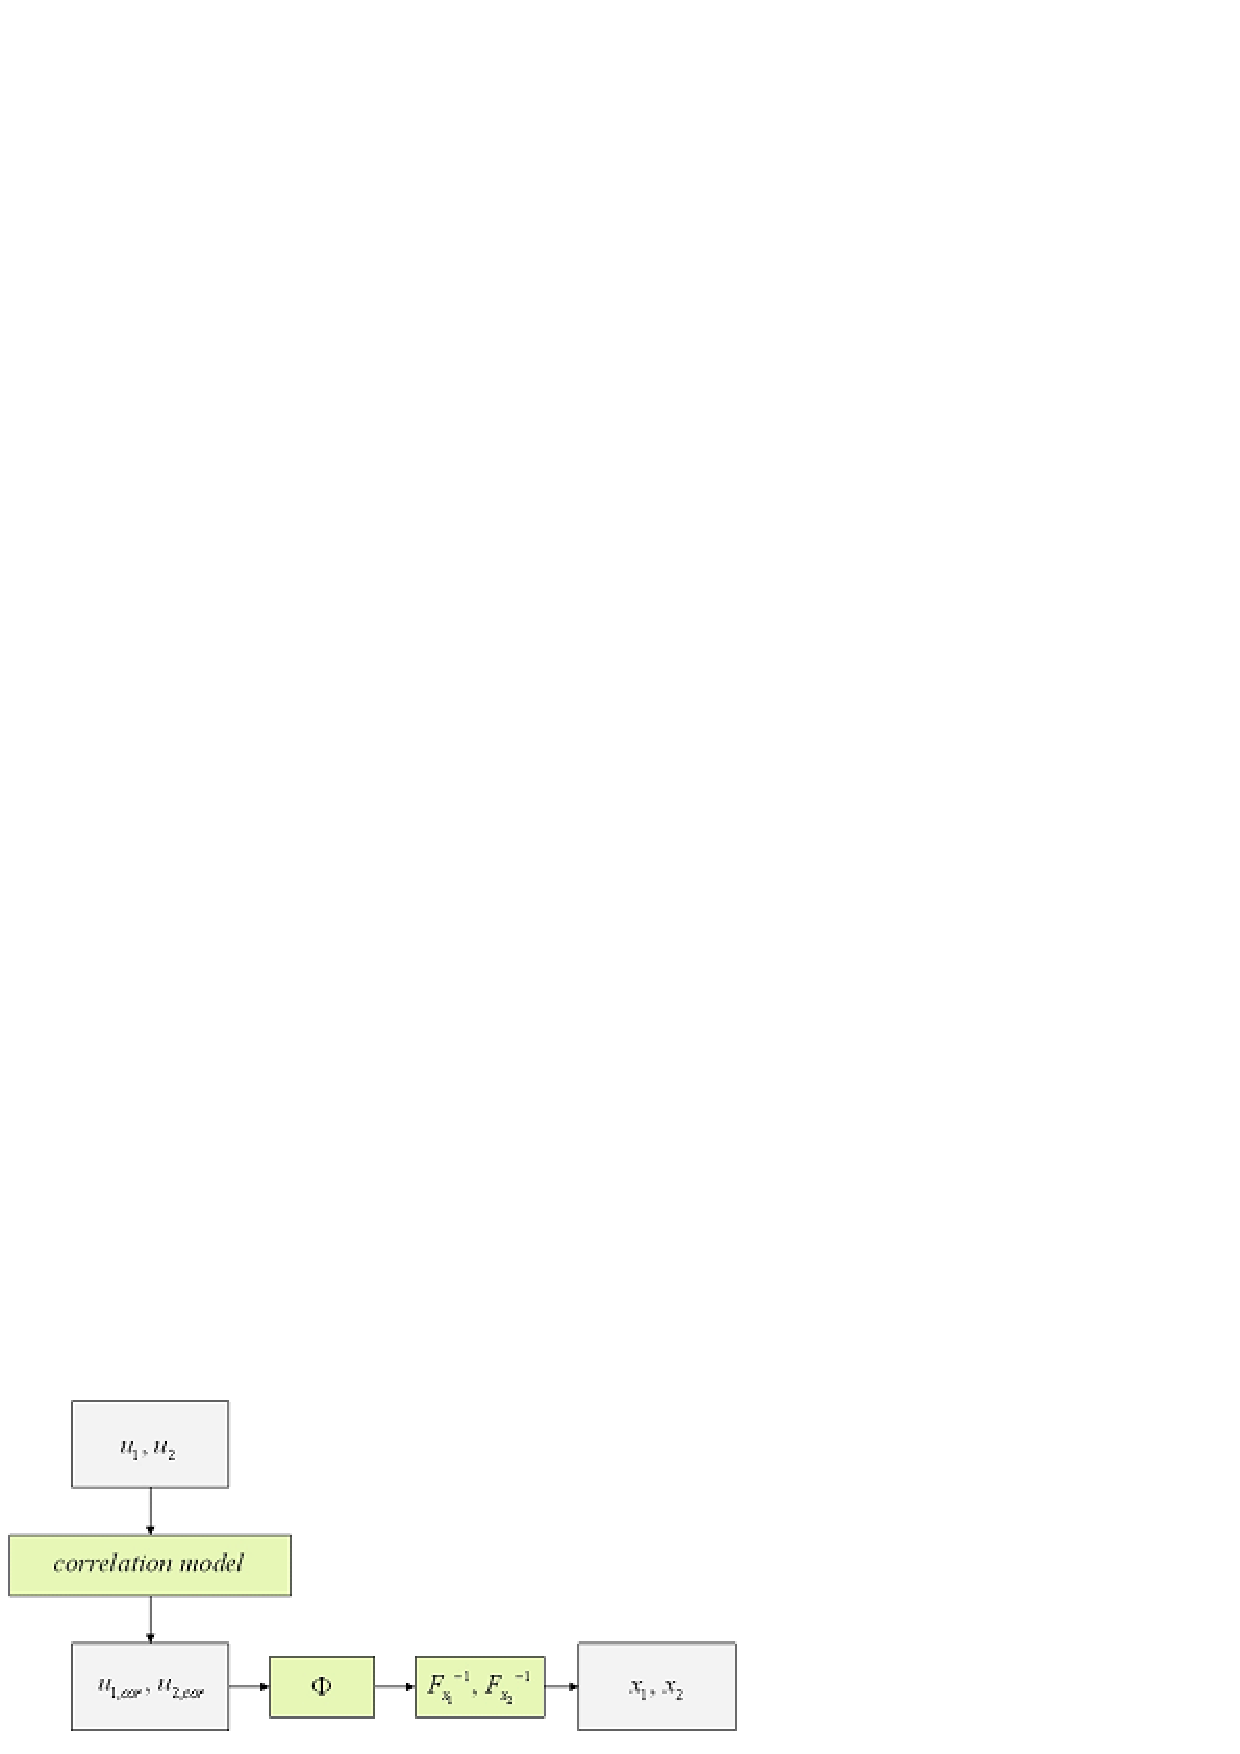
\includegraphics[width=1.0\columnwidth]{probabilisticLib_funcdesign_chapters/figloadmodels/image59.png}
\caption{Procedure for determining a load variable associated with randomly selected standard normally distributed variables for the case of correlated variables.}\label{fig:Figure_3.8}
\end{figure}

Since $U_{1,cor}$ and $U_{2,cor}$ are correlated variables, $X_1$ and $X_2$ are also correlated. Furthermore, since $U_{1,cor}$ and $U_{2,cor}$ are standard normally distributed and the translation from $U_{1,cor}$ and $U_{2,cor}$ to $X_1$ and $X_2$ is done in the exact same way as described in \Aref{Section_3.3}, it is automatically taken care of that $X_1$ and $X_2$ are distributed according to their prescribed distribution functions $F_{X_1}$ and $F_{X_2}$. The remainder of this section therefore focuses on the first part of the procedure: the generation of samples $u_{1,cor}$ and $u_{2,cor}$ of correlated variables $U_{1,cor}$ and $U_{2,cor}$.

The generation of $U_{1,cor}$ and $U_{2,cor}$ starts with the generation of realizations $u_1$ and $u_2$ of independent standard normally distributed random variables $U_1$ and $U_2$. Subsequently, $u_1$ is transformed into a sample $v$ of variable $V$ with distribution function $F_V(v)$. The transformation is done in similar style as explained in section \Aref{Section_3.3}, i.e. by making sure the probability of (non-)exceedance of $u_1$ and $v$ are equal: 
\begin{equation}
\Phi \left(u_{1} \right)=F_{V} \left(v\right)\Rightarrow v=F_{V} ^{-1} \left(\Phi \left(u_{1} \right)\right)\label{3.16)} 
\end{equation}

The $\Phi$ in this equation is the standard normal cumulative distribution function and $F_V(v)$ can be any cumulative distribution function, such as the normal, uniform or exponential distribution distribution. Subsequently, a sample $w$ is introduced that is dependent on $v$ and on a sample $u_2$ from a second standard normally distributed variable $U_2$:
\begin{equation} 
w=G\left(v,u_{2} \right)\label{ZEqnNum327839}
\end{equation}

The $G$ in this equation is a function that determines the correlation between $v$ and $w$. Subsequently, $v$ and $w$ are transformed back into samples $u_{1,cor}$ and $u_{2,cor}$ of standard normally distributed variables $U_{1,cor}$ and $U_{2,cor}$ by using the inverse CDFs or probabilities of (non-)exceedance. This leads to a $u_{1,cor}$ that identical to $u_1$, but $u_{2,cor}$ will be different from $u_2$ because of the use of the correlation function $G$. 

\begin{figure}[H]\centering
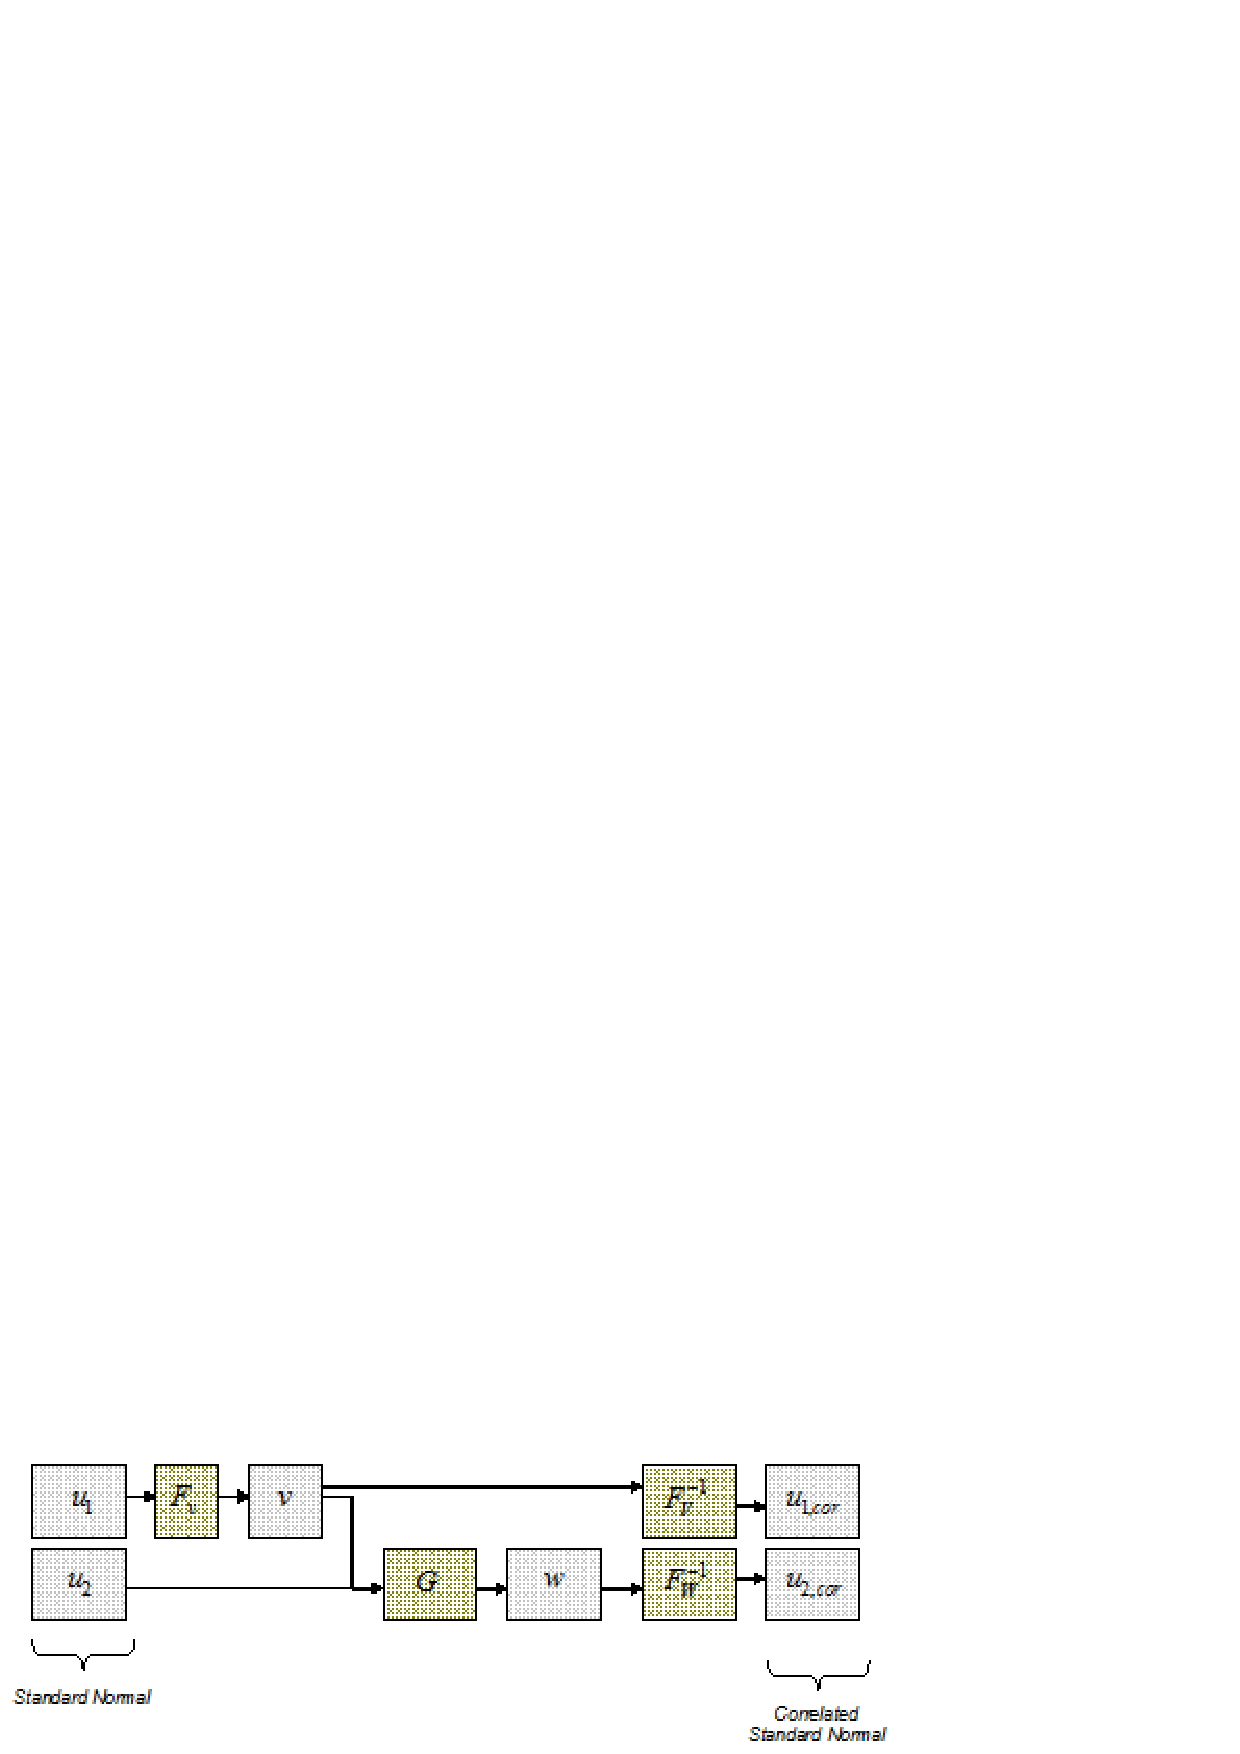
\includegraphics[width=1.0\columnwidth]{probabilisticLib_funcdesign_chapters/figloadmodels/image60.png}
\caption{Procedure for samples $u_{1,cor}$ and $u_{2,cor}$ of correlated standard uniform random variables $U_{1,cor}$ and $U_{2,cor}$.}\label{fig:Figure_3.9}
\end{figure}

The function $G$ is essentially the correlation model for variables $X_1$ and $X_2$. Many different functions $G$ can be used (note: $G$ is not a distribution function), also because the subsequent transformations $F_{V}^{-1}$ guarantee that $X_1$ and $X_2$ are distributed according to the pre-defined distribution functions $F_{X_1}$ and $F_{X_2}$. 
Naturally, function $G$ should be chosen such that it reproduces the observed correlation between variables $X_1$ and $X_2$ as well as possible. For a more detailed background on the derivation and application of correlation models in flood risk analysis, the interested reader is referred to the paper of \cite{Diermanse_Geerse_2012}. 

\section{Correlation models}\label{Section_3.4.2}

The following bi-variate correlation models are addressed in this section:
\begin{itemize}
\item Complete correlation,
\item PCR correlation model,
\item Volker correlation model,
\item HES correlation model,
\item Gaussian correlation model.
\end{itemize}
The complete correlation model is trivial as in this model $u_{2,cor}=u_{1,cor}=u_{1}$, this model will not be described any further. 

The PCR model is related to the Heteroscedastic (HES) model. Therefore a description of the PCR model in \Aref{Section_3.4.2.2} is preceded by a description of the HES model in \Aref{Section_3.4.2.3}. 

The Volker model is used to describe the wind-sea water level statistics in the tidal river areas. For a description of the Volker model, the reader is referred to \cite{basistochasten2017}. 

The bi-variate Gaussian correlation model has been implemented for practical purposes and it is described in \Aref{Gaussian_correlation_model}. The correlation model is a special case of the Gaussian copula model: the Gaussian copula model with $2$ variables gives the same results as the bi-variate Gaussian correlation model. The Gaussian copula model for $\geq 2$ random variables is described in \Aref{Gaussian_copula_model}. 

\subsection{HES correlation model}\label{Section_3.4.2.2}
The HES model is shorthand for ''Heteroscedastic model'', which means that the correlation varies depending on the values of $X_1$ and $X_2$. The model is very flexible and allows the user to set up a broad range of correlation structures. The model is described in the paper of \cite{Diermanse_Geerse_2012} and it is also referred to as the 'NL-model'.

The model describes the correlation between two random variables, $X_1$ and $X_2$ derived from two standard normal random variables $U_1$ and $U_2$. In the model, $U_1$ is the independent variable and $U_2$ the dependent variable (see \Fref{fig:Figure_3.9} for reference). 

The first step in the model is to transform the independent variable, $U_1$, sample $u_1$, into a standard exponentially distributed variable $V$, realization $v$.
\begin{equation} 
v=F_{V} ^{-1} \left(\Phi \left(u_{1} \right)\right)=-\ln \left(1-\Phi \left(u_{1} \right)\right)\label{ZEqnNum667656}
\end{equation}

The transformation is such that $v$ and $u_1$ have the same probability of (non-)exceedance (see \Aref{Section_2.2.3} for more information on this type of transformations). 

The next step is to compute the realization, $w$, of the dependent variable $W$. To describe the computation of $w$, first a couple of definitions are given. Let $\lambda (t)$ be a probability density function with a mean of $0$ and a standard deviation of $1$. This can be, but does not necessarily need to be, a standard normal density function. From $\lambda (t)$, distributions of the same type, but with different standard deviations, can be derived through the following transformation:
\begin{equation}
\lambda _{\sigma } \left(t\right)=\frac{1}{\sigma } \lambda \left({t\mathord{\left/ {\vphantom {t \sigma }} \right. \kern-\nulldelimiterspace} \sigma } \right)\label{3.19)}
\end{equation}

Density function $\lambda_{\sigma} (t)$ has a mean of $0$ and a standard deviation equal to $\sigma $. The cumulative distribution function, $\Lambda_{\sigma}$, is:
\begin{equation} 
\Lambda _{\sigma } \left(t\right)=\Lambda \left({t\mathord{\left/ {\vphantom {t \sigma }} \right. \kern-\nulldelimiterspace} \sigma } \right) \label{3.20)}
\end{equation}

The value of $w$ is computed as a combination of the realization $v$ of independent variable $V$ (correlated part) and of the realization $u_2$ of the standard normal variable $U_2$ (uncorrelated part):
\begin{equation}
w=v+\delta +\Lambda _{\sigma \left(v \right)}^{-1} \left(\Phi \left(u_{2} \right)\right)\label{ZEqnNum481579}
\end{equation}

Where $\delta$ is an offset that can be chosen arbitrarily and $\Lambda_{\sigma \left(v \right)}^{-1}$ is the inverse of the CDF of the uncorrelated part, with a $\sigma$ that can depend on the value of $v$. 
The right hand side of this equation is essentially the description of function $G$ of formula \eqref{ZEqnNum327839}, see \Fref{fig:Figure_3.9}. A schematic graph of the relationship between $w$ and $v$ is shown in \Fref{fig:Figure_3.10}. The dashed line shows the correlated part of the relationship between $v$ and $w$. The distribution around that line, in this case a normal distribution, is shown for two values of $v$. Note that in \Fref{fig:Figure_3.10} the standard deviation can vary with $v$. That is, for increasing values of $v$, the standard deviation of $w$ values around $v$ can increase or decrease. 
For a constant variance of $w$ for all $v$, $\sigma (v)$ is simply set constant. The relationship $\sigma (v)$ needs to be determined a-priori and included as input in the correlation model. The procedure to determine $\sigma (v)$ is an iterative one, and is described in \cite{Diermanse_Geerse_2012}. 

\Note{when $\Lambda _{\sigma(v)}$ is normally distributed with constant standard deviation $\sigma(v)=\sigma>0$, then equation \eqref{ZEqnNum481579} simplifies to $w=v+\delta+\sigma u_{2}$. This special case of the HES model is called the Constant Spread (CS) correlation model.}

\begin{figure}[H]\centering
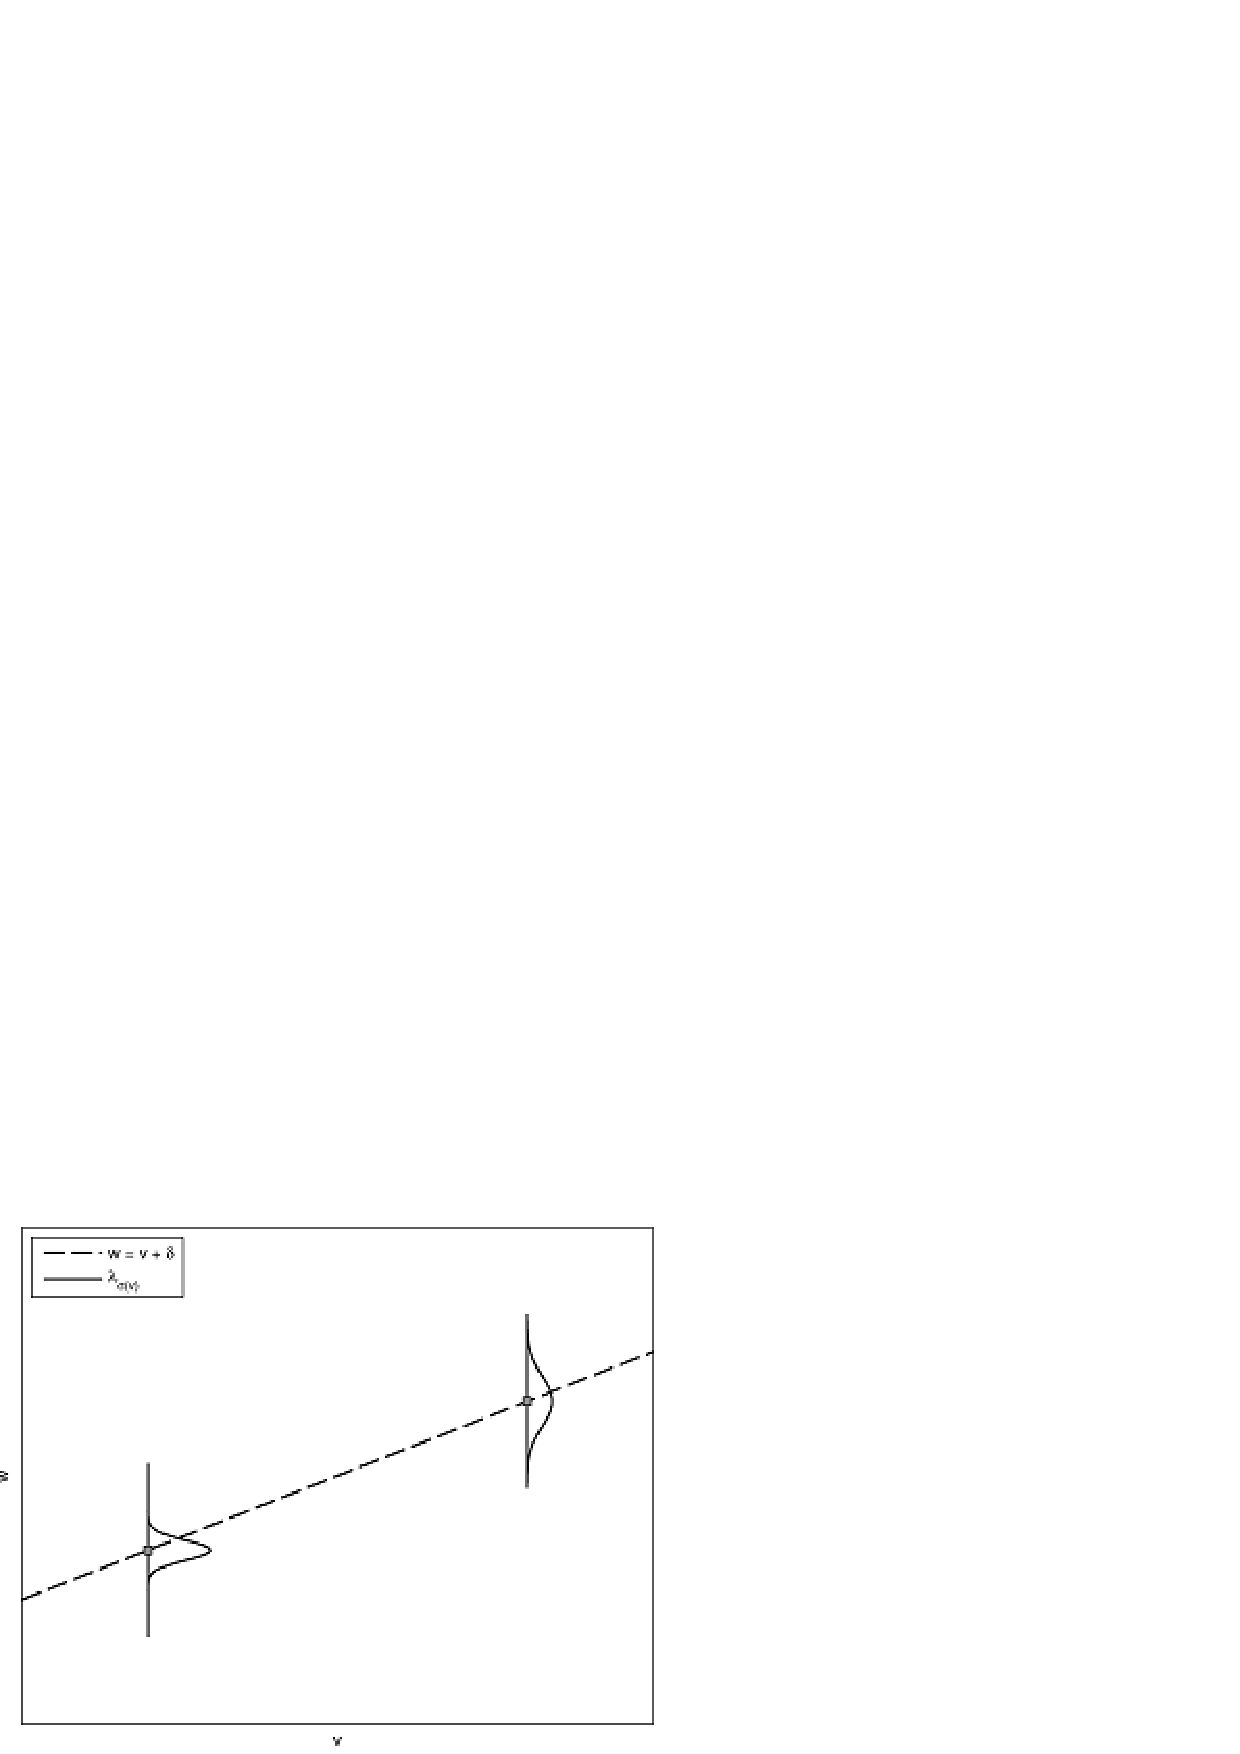
\includegraphics[width=0.8\columnwidth]{probabilisticLib_funcdesign_chapters/figloadmodels/image61.png}
\caption{Schematic illustrating the relationship between $w$, $v$, and $u_2$ in the NL model.}\label{fig:Figure_3.10}
\end{figure}

The next step in the correlation model is to transform the variables $V$ and $W$ back to standard normal variables $U_{1,cor}$ and $U_{2,cor}$. For this purpose, the distribution functions $F_V(v)$ and $F_W(w)$ are required. 
The transformation from $V$ to $U_{1,cor}$ is done as follows:
\begin{equation}
u_{1,cor} =\Phi ^{-1} \left(F_{V} \left(v\right)\right)=\Phi ^{-1} \left(1-e^{-v} \right)\label{3.22)}
\end{equation}

This transformation is the inverse of the transformation in equation \eqref{ZEqnNum667656}. This leads to a $u_{1,cor}$ that is exactly the same as $u_1$. 

The transformation from $W$ to $U_{2,cor}$ is done as follows:
\begin{equation} 
u_{2,cor} =\Phi ^{-1} \left(F_{W} \left(w\right)\right)\label{ZEqnNum307043} 
\end{equation}

This is generally less straightforward because there is often no analytical description available of the distribution function $F_W(w)$. The distribution can be derived from the following integral (according to the theorem of total probability):
\begin{equation} 
F_{w} \left(w\right)=\int _{0}^{\infty }f_{V} \left(v\right)P\left[W<w\left|v\right. \right]dv= \int _{0}^{\infty }\exp \left(-v\right)\Lambda _{\sigma \left(v\right)} \left(w-v-\delta \right)dv \label{ZEqnNum141107}
\end{equation}

\subsection{PCR correlation model}\label{Section_3.4.2.3}
The correlation model referred to as PCR (PC-Ring) is given this naming convention because it is the correlation model which was developed and used as the standard correlation model in PC-Ring. The model is similar to the HES, except that it includes a simplifying approximation for reasons of computational efficiency. The assumption is that variable $W$ is exponentially distributed, which means that the transformation \eqref{ZEqnNum307043} can be done without the numerical integration of equation \eqref{ZEqnNum141107} . The reduction in computation time was valuable in the period that PC-Ring was developed. 

Just as the HES model, the PCR model has an independent variable $V$ and a dependent variable $W$. $V$ is once again standard exponentially distributed and the realizations $v$ of this variable can be derived using equation \eqref{ZEqnNum667656}. 

Realizations of variable $W$ are derived using equation \eqref{ZEqnNum481579}. However, because of the assumption of exponentially distributed $W$, the parameter $\delta$ and function $\Lambda$ are given by:
\begin{equation}
\delta=-\frac{\sigma ^{2} }{2}
\end{equation}
and 
\begin{equation}
\Lambda _{\sigma \left(v \right)}^{-1} \left(\Phi \left(u_{2} \right)\right) = \sigma u_{2} 
\end{equation}
So:
\begin{equation}
w=v-\frac{\sigma ^{2} }{2} +\sigma u_{2} \label{ZEqnNum466239}
\end{equation}

In the PCR model, parameter $\sigma$ determines the measure of correlation. Small values of $\sigma$ correspond to a strong correlation, whereas large values of $\sigma$ correspond to weak correlation. 

\Fref{fig:Figure_3.11} shows the assumed probability density function of variable $W$ in the PCR model, i.e the standard exponential density function. Furthermore, it shows the probability density function of the HES model, $f_W(w)$, in case of a constant standard deviation. As can be seen, $f_W(w)$ converges to the standard exponential density function in the right tail. In other words: for larger values of $w$, variable $W$ of the HES model with constant correlation is (asymptotically) standard exponentially distributed. 

As mentioned, the PCR model assumes that the variable $W$ is standard exponentially distributed over the entire domain. This means the transformation from variable $W$ to the standard normal variable $U_{2,cor}$ is done by:
\begin{equation} 
u_{2,cor} =\Phi ^{-1} \left(F_{W} \left(w\right)\right)=\Phi ^{-1} \left(1-e^{-w} \right)\label{ZEqnNum122862}
\end{equation}

Since equation \eqref{ZEqnNum122862} is much easier to solve than equations \eqref{ZEqnNum141107} and \eqref{ZEqnNum307043}, the PCR-model requires less computation time than the HES model. However, by making the assumption of a standard exponential distribution function, the PCR-model introduces an error for small $w$, as can be seen in \Fref{fig:Figure_3.11}. This error will propagate in the value of $u_{2,cor}$ and eventually also in $x_2$, i.e. the realization of the associated ''real-world'' variable $X_2$. The reason why the assumption of the PCR model is reasonable is that for failure computations only large values of load variables are relevant and the error introduced by the assumption is generally negligible. 

\Note{this assumption can become less sound when smaller values of the load variables are relevant for failure as well. For instance at a location near the sea in a tidal river system, failure (flooding) most likely occurs during an event with extremely high sea water levels in combination with ''average'' river discharges. If the river discharge is estimated from the PCR model, errors may be introduced in estimating the probability of occurrence of such an event. However an analysis of the consequences has shown the practical effects on calculated water levels are marginal.

\begin{figure}[H]\centering
\includegraphics*[width=4.16in, height=3.27in, keepaspectratio=false]{probabilisticLib_funcdesign_chapters/figloadmodels/image62.png}
\caption{Probability density function of variable $W$ in the PCR-model, compared with the density function of a standard exponential distribution function.}\label{fig:Figure_3.11}
\end{figure}

\subsection{Gaussian correlation model}\label{Gaussian_correlation_model}
This section describes the bi-variate Gaussian correlation model that can be used to describe a simple correlation between standard normal random variables.
Given is the following correlation matrix $C$ with correlation coefficient $\rho\in[-1,1]$:
\begin{equation} 
C = \begin{bmatrix}
1.0 & \rho\\
\rho & 1.0\\
\end{bmatrix}
\end{equation} 

The 'lower' Cholesky decomposition of this matrix is (i.e. $P\times P^{T}=C$):
\begin{equation} 
P = \begin{bmatrix}
1.0 & 0.0\\
\rho & \sqrt{1-\rho^2}\\
\end{bmatrix}
\end{equation} 

Given an uncorrelated sample of standard normal random variables $u_1$ and $u_2$, the correlated sample $u_{1,cor}$ and $u_{2,cor}$ is derived as follows:
\begin{equation} 
[u_{1,cor},u_{2,cor}]=[u_1,u_2]\times P^{T} = [u_1,u_2]\times
\begin{bmatrix}
1.0 & \rho\\
0.0 & \sqrt{1-\rho^2}\\
\end{bmatrix}
\end{equation} 

This simplifies to:
\begin{equation} 
u_{1,cor}=u_1
\end{equation} 
and
\begin{equation} 
u_{2,cor}=u_1\rho+u_2\sqrt{1-\rho^2}
\end{equation}

The following figure pictures the uncorrelated and correlated samples for $\rho=0.5$.

\begin{figure}[H]\centering
\includegraphics*[width=4.16in, height=3.27in, keepaspectratio=false]{probabilisticLib_funcdesign_chapters/figsystemreliability/fig_gaussian_model.png}
\caption{Uncorrelated (left) and correlated (right) samples according to the Gaussian correlation model assuming $\rho=0.5$.}
\end{figure}

Furthermore, the following holds:
\begin{itemize}
\item When $\rho=0.0$ then the correlated sample is equal to the uncorrelated sample.
\item When $\rho=1.0$ then $u_{2,cor} = u_1$ (complete correlation).
\item When $\rho=-1.0$ then $u_{2,cor} = -u_1$ (reverse complete correlation).
\end{itemize}

\subsection{Gaussian copula model}\label{Gaussian_copula_model}
This section presents a Gaussian copula model, which can be used to describe correlation between $\geq 2$ variables in the $U$-space. The correlation coefficients are in this case stored in a correlation matrix.

A correlation matrix is a table showing correlation coefficients (i.e. product moment correlations) between variables. The diagonal of the table is always a set of ones, because the correlation between a variable and itself is always $1.0$. The matrix is also symmetric -- the correlation coefficient between variables $X$ and $Y$ is equal to the correlation coefficient between variables $Y$ and $X$. Moreover, the matrix must be positive definite, that is:
\begin{equation}
x^T\cdot C\cdot x>0 \mbox{ for all $x\in\Re^{n}\setminus\{0\}$ }
\end{equation}
where $C$ is a correlation matrix with size $n\times n$ and $T$ denotes the transpose.

In the \probLib, it is possible to describe correlations between random variables in a correlation matrix. The procedure to generate correlated samples $u_{cor}$ is as follows (see \cite{Diermanse_etal_2014}):
\begin{enumerate}
\item Derive a matrix $P$ for which $P\cdot P^{T}=C$ through Cholesky decomposition of correlation matrix $C$ with size $n\times n$ (see \cite{Strang_1982}).
\item Sample values $u_1,...,u_n$ from the standard normal distribution function and store the values in a $1\times n$ vector $u$.
\item The sample of the correlated standard normally distributed random variables $u_{cor}$ is then defined as follows: $u_{cor}=u\cdot P^{T}$.
\end{enumerate}

In the \probLib a special care is taken of correlation matrices with off-diagonal $\pm1.0$ elements. Such matrices usually do not satisfy the positive definite requirement. In order to perform calculations with such matrices, a two-step procedure is applied, during which the original matrix is decomposed into two matrices: (1) a matrix without the off-diagonal $\pm1.0$ elements and (2) a matrix with $0.0$ and $\pm1.0$ entries that indicate the positions of the off-diagonal $\pm1.0$ elements in the original matrix. The Cholesky decomposition is performed on the first matrix, highly increasing the chance that the positive definite requirement will be satisfied. The vector $u$ is first multiplied with the Cholesky decomposition matrix entailing a correlated sample without the full correlation cases. The resulting sample vector is then multiplied by the second matrix assuring that the same values are assigned to the fully correlated variables. The procedure is explained in more detail in the following example.

Consider the following correlation matrix $C$ with $\rho_{1,2}=\rho_{2,1}=1.0$:
\begin{equation} 
C = \begin{bmatrix}
1.0 & \rho_{1,2} & ... & \rho_{1,j} & ... & \rho_{1,n}\\
\rho_{2,1} & 1.0 & ... & \rho_{2,j} & ... &  \rho_{2,n}\\
... & ... & ... & ... & ...  & ...\\
\rho_{i,1} & \rho_{i,2} & ... & 1.0 & ... & \rho_{i,n}\\
... & ... & ... & ... & ...  & ...\\
\rho_{n,1} & \rho_{n,2} & ... & \rho_{n,j} & ... & 1.0\\
\end{bmatrix}
\end{equation} 

Matrix $C$ is decomposed into matrix $C_1$ and $C_2$. Matrix $C=C_1$ except for off-diagonal values found in the second row and column. These values are all equal to $0.0$. Matrix $C_2$ is an identity matrix except for the second row and column where $\rho_{2,1}=1.0$, $\rho_{i,2}=0.0$ for $i=1...n$ and $\rho_{2,j}=0.0$ for $j=2...n$. 
\begin{equation} 
C_1 = \begin{bmatrix}
1.0 & \mathbf{0.0} & ... & \rho_{1,j} & ... & \rho_{1,n}\\
\mathbf{0.0} & \mathbf{1.0} & ... & \mathbf{0.0} & ... &  \mathbf{0.0}\\
... & ... & ... & ... & ...  & ...\\
\rho_{i,1} & \mathbf{0.0} & ... & 1.0 & ... & \rho_{i,n}\\
... & ... & ... & ... & ...  & ...\\
\rho_{n,1} & \mathbf{0.0} & ... & \rho_{n,j} & ... & 1.0\\
\end{bmatrix}
\end{equation} 

\begin{equation} 
C_2 = \begin{bmatrix}
1.0 & \mathbf{0.0} & ... & 0.0 & ... & 0.0\\
\mathbf{1.0} & \mathbf{0.0} & ... & \mathbf{0.0} & ... &  \mathbf{0.0}\\
... & ... & ... & ... & ...  & ...\\
0.0 & \mathbf{0.0} & ... & 1.0 & ... & 0.0\\
... & ... & ... & ... & ...  & ...\\
0.0 & \mathbf{0.0} & ... & 0.0 & ... & 1.0\\
\end{bmatrix}
\end{equation} 

Assuming that $P$ is the Cholesky decomposition of matrix $C_1$, then the correlated sample $u_{cor}$ is derived as follows: 
\begin{equation} 
u_{cor}=u\cdot P^{T}\cdot C_2^{T}
\end{equation} 